\label {fs-experiments}

To prove the feasibility of the proposed framework we conducted a series of experiments. We show the efficiency and scalability of the distributed streaming dataflow on top of~\FlameStream\ processing system. Latency and throughput are used as performance metrics. We also demonstrate an achieved accuracy using a simple machine learning model. As a dataset, we used an open corpus of news articles from Russian media resource lenta.ru~\cite{lentaru}. This dataset contains about 700 000 documents, which are labeled by one of 90 different topics. In the experiments, we generated a stream consisted of articles from the dataset sorted by the time of publishing.

\begin{figure}[htbp]
  \centering
  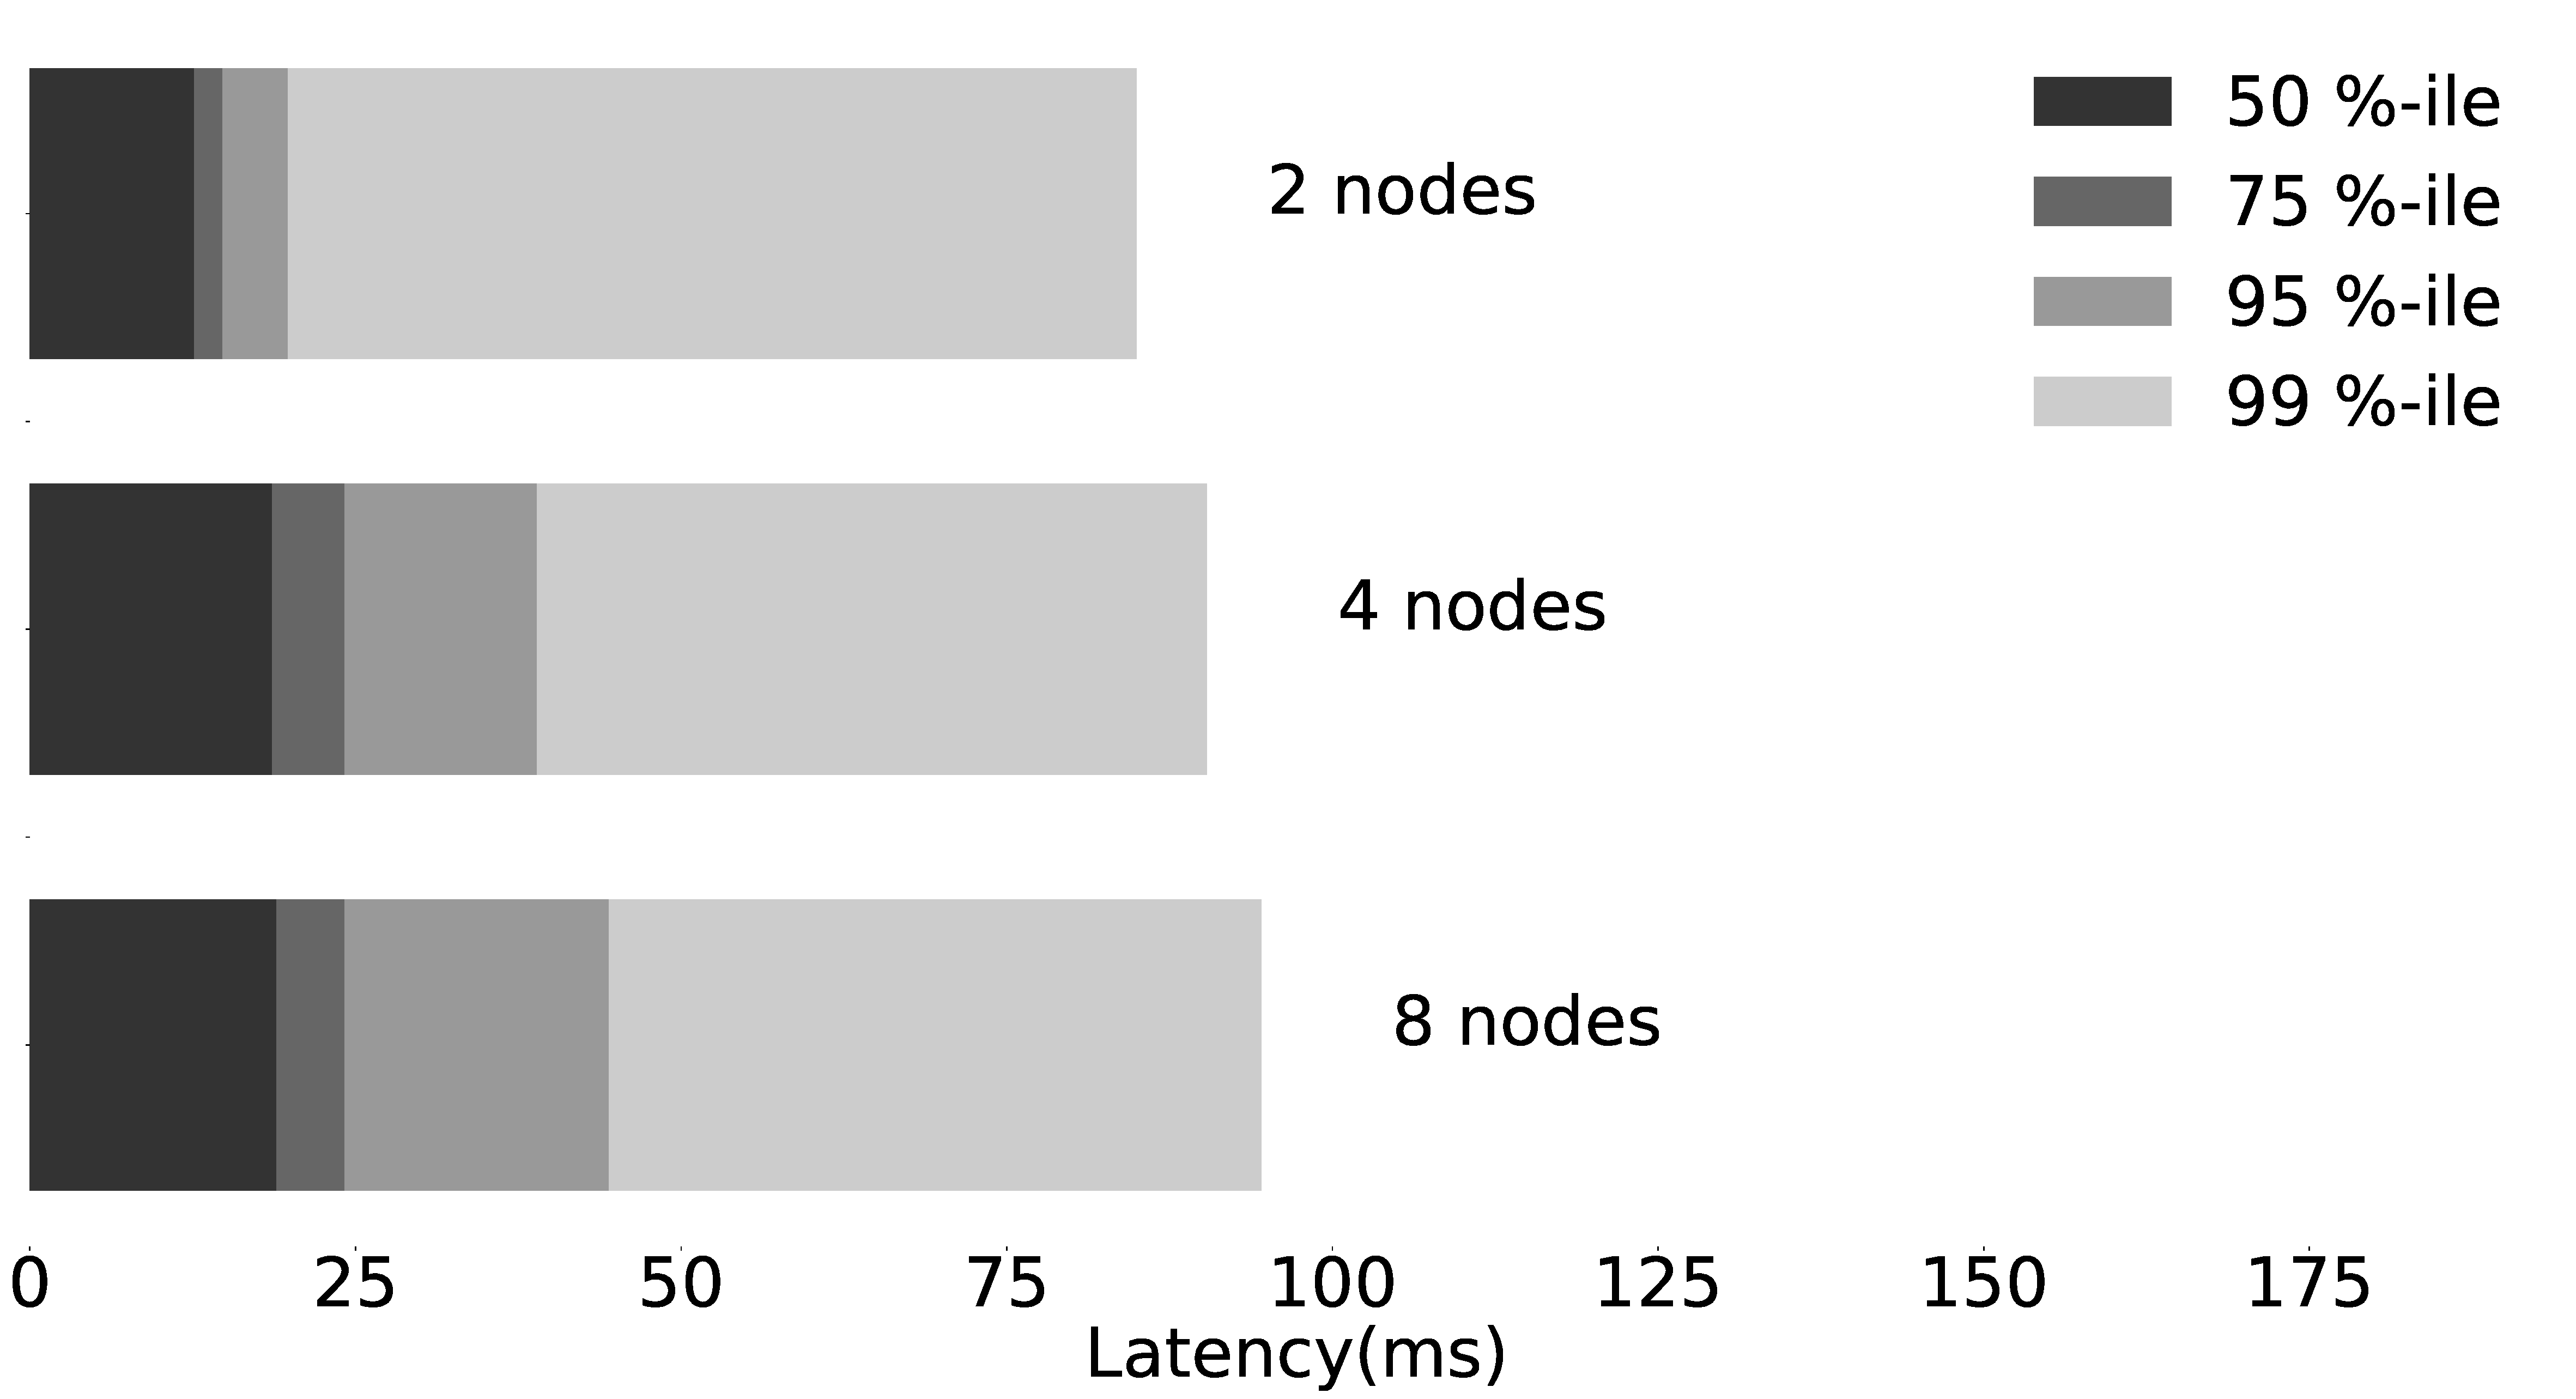
\includegraphics[scale=0.1]{pics/classifier_latencies}
  \caption{Classifier latencies}
  \label {latencies}
\end{figure}

\subsection{Data flow evaluation}

For evaluation, we deployed FlameStream on clusters, containing 2, 4 and 8 Amazon EC2 small instances with 2 GB of RAM and 1 core CPU. Exactly once guarantee was enabled. We measured throughput that is possible to achieve and the corresponding latency for prediction pipeline. We took into consideration only the performance of streaming pipeline without persistent queue. The results are shown in Figures~\ref{latencies} and~\ref{throughput}. As we can see, there is a linear trend in throughput, which proves the scalability of the framework. On the other hand, one can observe, that latency increases moderately and keeps under 25 ms for a median and under 100 ms for 99th percentile.

\begin{figure}[htbp]
  \centering
  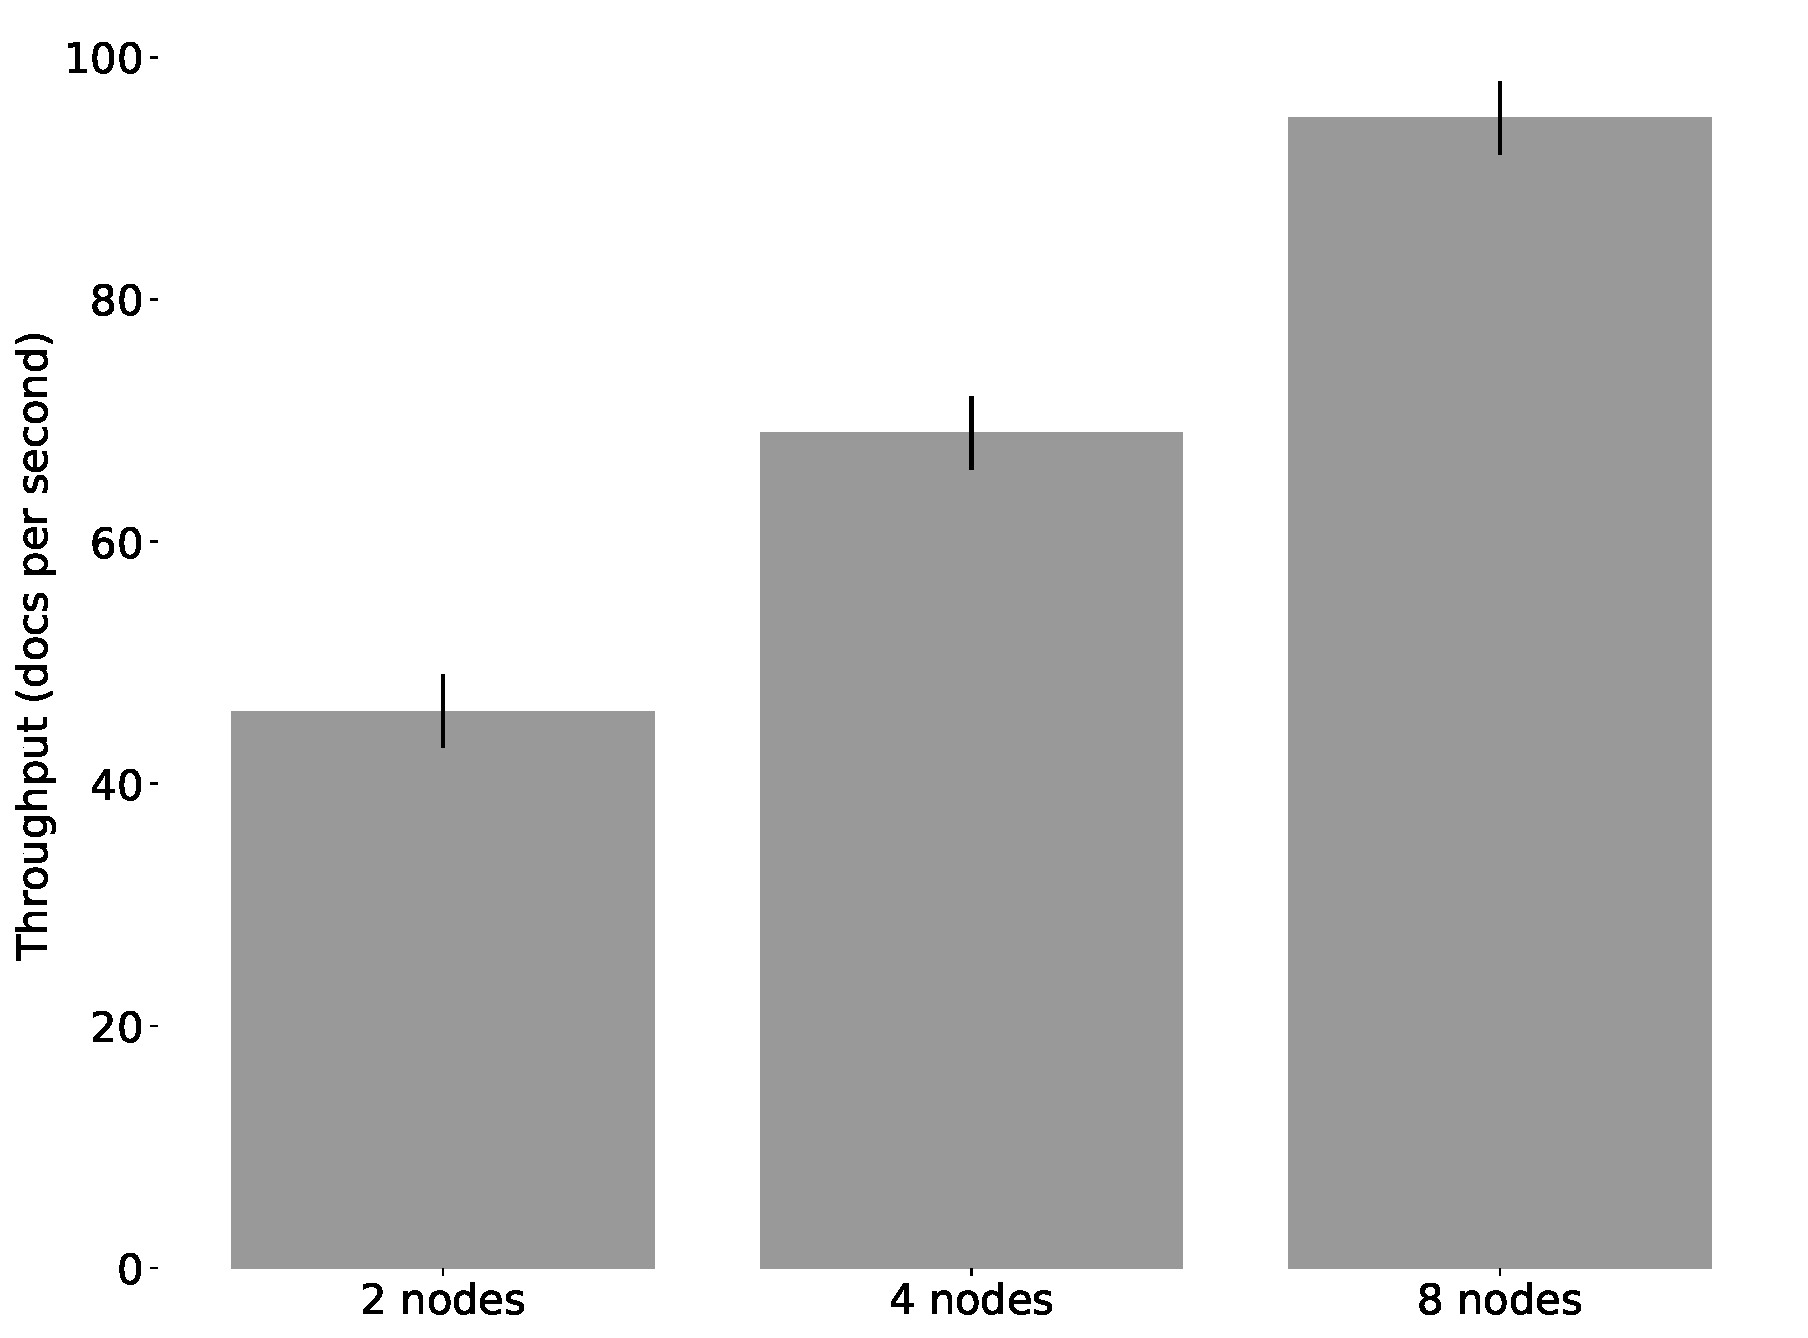
\includegraphics[scale=0.25]{pics/classifier_throughput}
  \caption{Classifier throughput}
  \label {throughput}
\end{figure}

\subsection{Classifier evaluation}

In order to be efficiently embedded in the proposed data flow, several properties of the machine learning model are desirable:
\begin{itemize}
     \item Small size of the model for storing and updating it in reasonable time and space.
     \item A possibility to update model with a new data.
\end{itemize}

We use Multinomial Logistic Regression as a training method. Model parameters (weights) are denoted as $W$. The training process is the maximization of the following formula in terms of $W$:

$$ logP(W | X) = \frac{1}{|X|} \sum \limits_{(x, y) \in X} \log \frac{e^{{W_y^T \cdot \; x}}}{\sum \limits_{l = 1}^{k}  e^{{W_{l}^T \cdot \; x}}} - \lambda_1 ||W||_1 - \lambda_2 ||W - W_{prev}||_2 $$ 

$X$ denoted as a training dataset and the number of classes is $k$. For changing the model over time, we use weights that computed in the previous step -- $W_{prev}$. At the first step, $W_{prev}$ can be provided by a pre-train process.

The first component is the standard softmax function for multiple classes. The second component keeps the $L1$ regularization of the weights, and provides sparsity, hence, the model has a small size -- about 1 Mb. We apply $L2$ regularization as the third component in order to use previous weights for on-the-fly model update.

We compared two approaches to the performance demonstration of the proposed machine learning model. The first one is training on the complete dataset with applying the formula, where $\lambda_2 = 0$. The approach does not use the history of the weights, therefore we denote it as a {\em static training}. The second one consists in dividing training dataset into relatively small batches and consequent applying MLR with $l2$ regularization to each batch. The latter case demonstrates the behavior of our streaming classification approach. The results are shown in Table~\ref{accuracy}. Streaming approach performance is slightly better than the first one. It indicates that our framework is able to handle the streaming nature of the news dataset including concept drift. The more formal rationale behind this fact is out of the scope of this paper and relates to our future work.

\begin{table}[htbp]
\begin{tabular}{lc}
Method             & Accuracy \% \\
Static training    & 0.667       \\
Streaming training & 0.671         
\end{tabular}
\caption{Accuracy comparison between static and stream training}
\label{accuracy}
\vspace{-7mm}
\end{table}